\documentclass[11pt,a4paper]{article}
\usepackage[T1]{fontenc}
\usepackage[utf8]{inputenc}
\usepackage{amsmath,amssymb,amsthm}
\usepackage[margin=2.6cm]{geometry}
\usepackage{booktabs}
\usepackage{float}
\usepackage{graphicx}
\graphicspath{{figs/}{../figs/}}
\usepackage[colorlinks=true,linkcolor=black,citecolor=black,urlcolor=black]{hyperref}

\renewcommand{\theequation}{C.\arabic{equation}}
\newcommand{\R}{\mathbb{R}}
\newcommand{\E}{\mathbb{E}}
\newcommand{\KL}{\mathrm{KL}}
\newcommand{\DEP}{\mathrm{DEP}}
\newcommand{\diag}{\operatorname{diag}}
\newcommand{\Neff}{N_{\mathrm{eff}}}
\newcommand{\dd}{\mathrm{d}}

\title{\large\bfseries Il laboratorio numerico della diagnostica a minimo d'azione\\[2pt]
\normalsize\mdseries contenuto economico dei risultati e struttura del codice\\[4pt]
\normalsize\itshape nota di accompagnamento al repository della tesi \emph{Diagnostica a minimo d'azione\\ della cattiva specificazione distributiva nei modelli HANK}}
\author{\normalsize Francesco Pinna\\ \normalsize Dipartimento di Economia e Finanza, LUISS Guido Carli}
\date{\normalsize 21 settembre 2026}

\renewcommand{\figurename}{Figura}
\renewcommand{\tablename}{Tabella}
\renewcommand{\abstractname}{Sommario}

\begin{document}
\maketitle

\begin{abstract}
\noindent Il codice raccolto nel repository riproduce un esperimento controllato su un'economia a un solo asset, nel quale una cattiva specificazione nota del processo di reddito viene iniettata in una regione nota della distribuzione della ricchezza e la diagnostica deve ritrovarla a partire dalla sola risposta del consumo. Letti in chiave economica, i risultati indicano che la risposta aggregata del consumo rende visibili le due code della distribuzione e quasi invisibile la sua parte centrale, che un aumento uniforme della frequenza delle transizioni di reddito è pressoché indistinguibile, sui soli aggregati, da una revisione di segno opposto del sentiero del tasso, e che l'aggiunta di pochi momenti sul consumo della metà meno ricca della popolazione scioglie questo confondimento perché i due meccanismi lasciano impronte distributive incompatibili. L'esercizio è in equilibrio parziale e la sua deformazione non separa un effetto sul reddito atteso da un effetto sul rischio, due limiti che coincidono con il lavoro della tesi.
\end{abstract}

\section{L'oggetto dell'esercizio}\label{sec:oggetto}
La domanda a cui il laboratorio risponde è se la risposta del consumo a uno shock contenga informazione sufficiente a stabilire in quale regione della distribuzione della ricchezza un modello ad agenti eterogenei rappresenti male il rischio di reddito affrontato dalle famiglie. Per rispondere occorre conoscere la risposta corretta, e per questo l'esercizio procede per iniezione, alterando deliberatamente il processo di reddito di un gruppo noto di famiglie, calcolando la risposta del consumo che ne risulta, e chiedendo alla diagnostica di attribuire lo scarto rispetto al modello di riferimento. Gli esperimenti sono privi di rumore campionario, sicché i residui dei momenti sono esatti e ogni errore di attribuzione va imputato alla sola geometria del problema.

Rispetto alla proposta di tesi, il laboratorio esercita il blocco delle famiglie in isolamento. Lo Jacobiano che vi compare è la sensibilità diretta dei momenti ai controlli a sentiero del tasso assegnato, cioè il termine $J_h$ della proposta, mentre il termine di retroazione di equilibrio $J_m(I-D_m\Phi)^{-1}D_h\Phi$ è assente perché il tasso è esogeno e non esiste condizione di market clearing. La chiusura dell'equilibrio costituisce il primo passo della tesi.

\section{L'economia di riferimento}\label{sec:economia}
Il modello è il blocco consumo--risparmio di un'economia alla Aiyagari (1994) a frequenza trimestrale. Le famiglie hanno utilità a elasticità costante con avversione al rischio $\gamma=2$ e fattore di sconto $\beta=0{,}97$, il tasso reale è $r=0{,}01$, il vincolo di indebitamento è $a\ge0$, e il reddito da lavoro segue una catena di Markov a due stati $y\in\{0{,}70;\,1{,}30\}$ con probabilità di permanenza $0{,}925$ in ciascuno stato. La politica di consumo è calcolata con il metodo della griglia endogena di Carroll (2006) su $120$ punti e la distribuzione evolve con le lotterie di Young (2010). L'economia è deliberatamente povera di attività, con una ricchezza aggregata pari a circa $1{,}5$ trimestri di reddito medio, perché la trasmissione che interessa a un modello HANK si concentra sulle famiglie vicine al vincolo e questa calibrazione ne produce una massa ampia.

\begin{table}[t]
\centering\small
\caption{Descrittori per quartile di ricchezza nello stato stazionario. Propensione marginale trimestrale al consumo da un trasferimento e quota di ricchezza sono calcolate sulla distribuzione di inizio periodo. La quota a reddito alto è calcolata sulla distribuzione di fine periodo, che è quella su cui agisce la deformazione.}
\label{tab:quartili}
\begin{tabular}{lcccc}
\toprule
 & $Q_1$ & $Q_2$ & $Q_3$ & $Q_4$\\
\midrule
propensione marginale al consumo & $0{,}80$ & $0{,}11$ & $0{,}06$ & $0{,}05$\\
quota della ricchezza aggregata & $0{,}004$ & $0{,}119$ & $0{,}305$ & $0{,}573$\\
quota di famiglie a reddito alto & $0{,}00$ & $0{,}47$ & $0{,}69$ & $0{,}86$\\
attività di fine periodo & $[0;\,0{,}19]$ & $[0{,}24;\,1{,}21]$ & $[1{,}34;\,2{,}43]$ & $[2{,}62;\,60]$\\
\bottomrule
\end{tabular}
\end{table}

Lo stato stazionario presenta una massa al vincolo pari a $0{,}191$, composta quasi interamente da famiglie nello stato di reddito basso, e una propensione marginale trimestrale media al consumo di $0{,}26$. La Tabella~\ref{tab:quartili} mostra la struttura che governa tutti i risultati successivi. Il primo quartile consuma l'$80$ per cento di un trasferimento entro il trimestre e detiene una quota trascurabile della ricchezza, il quarto ne consuma il $5$ per cento e detiene il $57$ per cento delle attività, e la composizione per stato di reddito varia in modo monotono lungo la distribuzione, dalla totale assenza di famiglie a reddito alto nel primo quartile a una quota dell'$86$ per cento nel quarto.

\section{La deformazione e il suo contenuto economico}\label{sec:deformazione}
Il controllo agisce sulle probabilità di cambiare stato di reddito. Per le famiglie la cui ricchezza di fine periodo $a'$ appartiene alla regione $\mathcal{A}_k$, le probabilità di transizione fuori diagonale sono moltiplicate per un fattore comune,
\begin{equation}\label{eq:tilt}
\Pi_{zz'}\;\longmapsto\;\big(1+\delta_k(t)\big)\,\Pi_{zz'},\qquad z'\neq z,\qquad a'\in\mathcal{A}_k,
\end{equation}
e la diagonale è rinormalizzata. Qui $\delta_k(t)$ è uno scalare, la variazione relativa al tempo $t$ della probabilità di cambiare stato per le famiglie della regione $k$, e le regioni sono quantili di ricchezza di uguale massa. Un valore positivo di $\delta_k$ aumenta la frequenza con cui le famiglie della regione cambiano stato di reddito, che nel seguito chiamo churn, e ne riduce corrispondentemente la persistenza.

Il contenuto economico di questa deformazione dipende dalla composizione della regione per stato di reddito, ed è questo il primo fatto che il laboratorio rende visibile. Nel primo quartile, dove le famiglie a reddito alto sono praticamente assenti, un aumento del churn opera come un aumento della probabilità di uscire dallo stato di reddito basso e quindi come un miglioramento delle prospettive di reddito per famiglie con propensione marginale elevata. Nel quarto quartile, dove prevalgono le famiglie a reddito alto, la stessa deformazione aumenta soprattutto la probabilità di perdere il reddito alto e opera come un peggioramento delle prospettive per chi detiene la maggior parte della ricchezza. Nel secondo quartile, dove i due stati sono quasi equamente rappresentati, gli effetti sul reddito atteso della regione si compensano e resta sostanzialmente la variazione della persistenza, cioè la componente più vicina a una deformazione di puro rischio.

La Figura~\ref{fig:economia}, pannello (a), riporta la risposta del consumo aggregato a un aumento del churn di ampiezza iniziale pari al $15$ per cento che decade al tasso trimestrale $0{,}85$, iniettato separatamente in ciascun quartile. L'aumento nel primo quartile innalza il consumo in modo crescente fino a un picco di $0{,}33$ punti percentuali otto trimestri dopo l'impatto, un profilo che riflette l'uscita progressiva dallo stato di reddito basso di famiglie che consumano quasi tutto il reddito aggiuntivo. Gli aumenti nel terzo e nel quarto quartile riducono il consumo di $0{,}10$ e $0{,}18$ punti fin dall'impatto, con profili quasi piatti, compatibili con una revisione immediata del reddito atteso da parte di famiglie che dispongono di ampie riserve. L'aumento nel secondo quartile produce una risposta di $0{,}03$ punti che si esaurisce rapidamente. La composizione suggerisce che nei quartili superiori il canale del reddito atteso pesi almeno quanto quello precauzionale, al quale l'appendice numerica di giugno attribuiva la risposta, e l'esperimento che separa i due canali è indicato nella Sezione~\ref{sec:limiti}.

\begin{figure}[t]
\centering
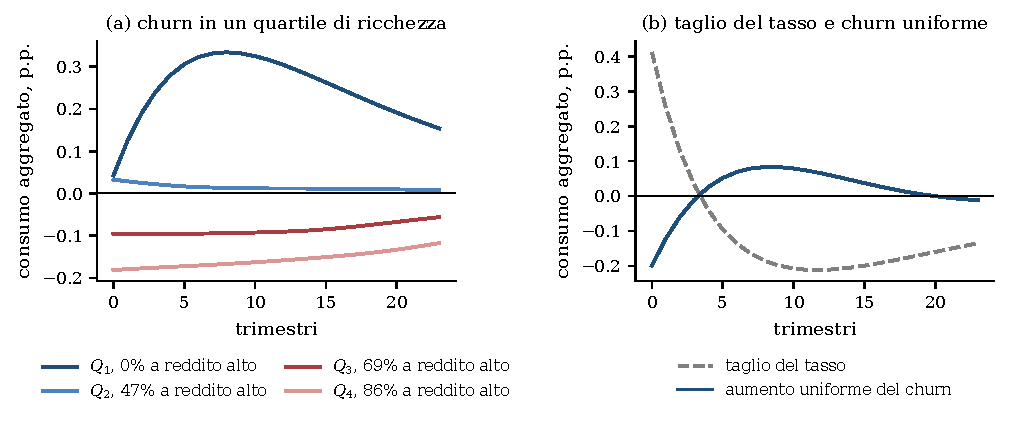
\includegraphics[width=\textwidth]{F0_economia.pdf}
\caption{(a) Risposta del consumo aggregato, in punti percentuali dello stazionario, a un aumento del churn $\delta_k(t)=0{,}15\cdot0{,}85^{\,t}$ nel quartile $k$ indicato, con la quota di famiglie a reddito alto nel quartile. (b) Risposta del consumo aggregato a un taglio anticipato del tasso $\dd r_t=-0{,}005\cdot0{,}8^{\,t}$ e a un aumento uniforme del churn sull'intera popolazione, entrambe calcolate sul sentiero non lineare.}
\label{fig:economia}
\end{figure}

\section{Il costo e la sua forma}\label{sec:costo}
Il costo di una deformazione è l'entropia relativa fra il processo di reddito deformato e quello di riferimento, sviluppata al secondo ordine. Per una famiglia che cambia stato con probabilità $p$ in un trimestre, portare tale probabilità a $p(1+\delta)$ costa
\begin{equation}\label{eq:bernoulli}
\KL\big(\mathrm{Bern}(p(1+\delta))\,\big\|\,\mathrm{Bern}(p)\big)\;=\;\frac{p\,\delta^2}{2(1-p)}\;+\;O(\delta^3),
\end{equation}
perché il baseline è un minimo dell'entropia relativa e la sua curvatura in quel punto è l'inverso della varianza della variabile di transizione. Il codice adotta la forma limite in tempo continuo, nella quale il peso è l'intensità $p$ stessa, coerentemente con la formulazione a intensità della proposta. Aggregando sulle famiglie della regione, il costo per trimestre della deformazione $\delta_k(t)$ è $\tfrac12\,\bar q_k\,\delta_k(t)^2$ per capita, dove
\begin{equation}\label{eq:qbar}
\bar q_k\;=\;\sum_{a'\in\mathcal{A}_k}\sum_{z}\mu^{\mathrm{fine}}(a',z)\,\big(1-\Pi_{zz}\big)
\end{equation}
è il numero atteso di transizioni di reddito che hanno origine nella regione, per famiglia e per trimestre, e $\mu^{\mathrm{fine}}$ è la distribuzione di fine periodo. Il contenuto economico del peso è diretto. Inclinare una regione costa in proporzione a quante transizioni di reddito vi avvengono effettivamente, sicché una regione poco popolata, o nella quale le famiglie cambiano stato raramente, non offre correzioni a basso costo. In questo esercizio la probabilità di cambiare stato è la stessa nei due stati, $\bar q_k$ vale circa $0{,}019$ in ciascun quartile e il peso si riduce alla massa della regione.

Il costo per capita va moltiplicato per $\Neff$, il numero di storie individuali indipendenti che i dati disciplinano, perché una deformazione imposta a $\Neff$ famiglie costa $\Neff$ volte quella imposta a una sola. Alla deformazione idiosincratica si affianca il canale aggregato, un sentiero di deviazioni del tasso $\dd r_t$ con costo $\tfrac12\sum_t(\dd r_t/\sigma_r)^2$ e $\sigma_r$ pari a $25$ punti base trimestrali. Raccolti tutti i sentieri di controllo nel vettore $\eta$, di dimensione $T(1+n_r)$ con $T=40$ trimestri e $n_r$ regioni, e indicata con $\Omega_\eta^{-1}$ la matrice diagonale di precisione a priori che ne raccoglie i pesi, il problema risolto dal codice è
\begin{equation}\label{eq:problema}
\min_{\eta}\;\tfrac12\,\eta'\,\Omega_\eta^{-1}\,\eta\;+\;\tfrac{\rho}{2}\,\big\|\hat g-J\eta\big\|^2,
\end{equation}
dove $\hat g\in\R^{H}$ è il residuo dei momenti, costituito da $H=24$ deviazioni trimestrali del consumo aggregato, $J$ è la matrice di dimensione $H\times T(1+n_r)$ delle risposte dei momenti ai controlli, e $\rho$ è la precisione attribuita ai momenti. Il pedice di $\Omega_\eta$ distingue questa covarianza a priori dei controlli dalla covarianza campionaria dei momenti, che nella proposta di tesi porta lo stesso simbolo. Con $\rho=128$ la parte del residuo che la correzione lascia inspiegata è in media pari al $5$ per cento della sua norma.

La soluzione è lineare nel residuo, $\eta^\star=M\hat g$ con $M=(\Omega_\eta^{-1}+\rho J'J)^{-1}\rho J'$, e il costo si decompone esattamente per blocchi,
\begin{equation}\label{eq:decomposizione}
I\;=\;\tfrac12\,\eta^{\star\prime}\,\Omega_\eta^{-1}\,\eta^\star\;=\;\sum_{b}I_b,\qquad s_b\;=\;\frac{I_b}{I},
\end{equation}
dove $b$ scorre il blocco aggregato e le $n_r$ regioni e $s_b$ è la quota del costo attribuita al blocco. La capacità $\bar s_b$ è la quota massima che il blocco può assorbire al variare del residuo, calcolata come massimo autovalore generalizzato della coppia di forme quadratiche che definiscono $I_b$ e $I$, e l'attribuzione usa la frazione di capacità utilizzata $u_b=s_b/\bar s_b$. Infine la probabilità di errore di rilevazione,
\begin{equation}\label{eq:dep}
\DEP\;=\;\Phi\big(-\sqrt{I/2}\,\big),
\end{equation}
traduce il costo nella probabilità di confondere il modello deformato con quello di riferimento, nella forma gaussiana usata da Hansen e Sargent (2008). Un valore prossimo a $0{,}5$ indica una deformazione che i momenti non permetterebbero di rilevare.

\section{Che cosa vede la risposta aggregata del consumo}\label{sec:aggregato}
La capacità misura quanta parte del costo di riconciliazione ciascun blocco può assorbire, e quindi quanto la risposta aggregata del consumo sia in grado di vedere una deformazione in quella regione. Con quattro regioni e $\Neff=8000$ le capacità valgono $0{,}931$ per il canale aggregato e $0{,}443$, $0{,}022$, $0{,}069$ e $0{,}277$ per i quattro quartili. Le code della distribuzione sono visibili e il centro è quasi invisibile, e la ragione è quella descritta nella Sezione~\ref{sec:deformazione}. Nel primo quartile la deformazione opera su famiglie con propensione marginale elevata, nel quarto su famiglie che detengono la maggior parte della ricchezza, mentre nel secondo quartile gli effetti sul reddito atteso si compensano e la risposta del consumo aggregato è minima. La regione nella quale la deformazione è più vicina a una variazione di puro rischio è quella che i consumi aggregati quasi non osservano.

Le iniezioni controllate confermano questa geometria. Un aumento del churn nel primo quartile produce un costo $I=2{,}12$ e una probabilità di errore di rilevazione di $0{,}15$, il $41$ per cento del costo è attribuito correttamente al primo quartile, ma un terzo si scarica sul canale aggregato e un quinto sul quarto quartile, perché le due code muovono il consumo aggregato con profili persistenti che il tasso può in parte imitare. Un'iniezione nel secondo quartile produce un costo di appena $0{,}016$ e una probabilità di errore di $0{,}465$, cioè una deformazione che questi momenti non permetterebbero in pratica di rilevare. In assenza di rumore la frazione di capacità utilizzata la attribuisce comunque alla regione corretta, un risultato che attesta l'assenza di distorsioni nella regola di attribuzione e che con dati reali resterebbe sepolto nella variabilità campionaria.

Il confronto con la regola alternativa ha un contenuto economico preciso. L'attribuzione basata sui contrasti fra coppie di blocchi assegna al quarto quartile sia l'iniezione nel secondo sia quella nel terzo, perché il quarto è il blocco con la risposta aggregata più ampia fra quelli di ricchezza elevata. Senza la normalizzazione per capacità, la diagnostica attribuirebbe sistematicamente la cattiva specificazione alle famiglie più ricche per la sola ragione che la loro impronta sul consumo aggregato è la più estesa.

Il secondo fatto rilevante riguarda il canale monetario. Il pannello (b) della Figura~\ref{fig:economia} mostra che un taglio anticipato del tasso di $50$ punti base innalza il consumo di $0{,}41$ punti all'impatto e lo porta sotto lo stazionario dopo quattro trimestri, fino a $-0{,}21$ punti dopo dodici, mentre un aumento uniforme del churn lo riduce di $0{,}20$ punti all'impatto e lo porta sopra lo stazionario dopo quattro trimestri. I due profili sono quasi speculari, con un coseno di $-0{,}86$ sui momenti aggregati. Una riduzione generalizzata del churn verrebbe dunque letta nella risposta del consumo aggregato come un allentamento monetario, e con una sola regione la diagnostica attribuisce l'iniezione di churn uniforme al canale del tasso con un margine ampio. Si tratta di un'attribuzione errata compiuta con sicurezza, il caso più insidioso per chi valuta la trasmissione sui soli aggregati.

\section{Il valore dei momenti distributivi}\label{sec:distributivi}
Il confondimento si scioglie aggiungendo ai momenti le deviazioni del consumo delle famiglie nella metà inferiore della distribuzione della ricchezza per dodici trimestri. Il taglio del tasso innalza il consumo di questo gruppo in modo marcato e persistente, da $0{,}29$ a circa $1{,}6$ punti, mentre l'aumento uniforme del churn produce una risposta più contenuta e a gobba. Sulla metà inferiore i due meccanismi si muovono nello stesso verso, con un coseno di $0{,}70$, mentre sugli aggregati si muovono in verso opposto. Una riduzione del churn che imitasse l'allentamento monetario sul consumo aggregato lo contraddirebbe quindi sul consumo della metà meno ricca, e il coseno complessivo scende a $0{,}58$.

\begin{table}[t]
\centering\small
\caption{Esito dell'attribuzione mediante frazione di capacità utilizzata per ciascun livello della famiglia annidata di regioni. Il margine è la distanza minima, sulle iniezioni, fra la frazione del blocco vero e quella del blocco concorrente più vicino.}
\label{tab:risoluzione}
\begin{tabular}{ccccc}
\toprule
 & \multicolumn{2}{c}{soli aggregati ($H=24$)} & \multicolumn{2}{c}{con la metà inferiore ($H=24+12$)}\\
\cmidrule(lr){2-3}\cmidrule(lr){4-5}
regioni $n_r$ & esito & margine & esito & margine\\
\midrule
$1$ & errato & $0{,}44$ & corretto & $0{,}79$\\
$2$ & corretto & $0{,}096$ & corretto & $0{,}35$\\
$4$ & corretto & $4{,}4\times10^{-6}$ & corretto & $0{,}092$\\
$8$ & errato & $2{,}4\times10^{-4}$ & errato & $5{,}6\times10^{-3}$\\
\bottomrule
\end{tabular}
\end{table}

La Tabella~\ref{tab:risoluzione} riassume l'effetto sull'intera famiglia di partizioni. Con i soli aggregati la partizione in quattro quartili è risolta con un margine di $4{,}4\times10^{-6}$, dovuto alla quasi indistinguibilità del terzo e del quarto quartile, le cui risposte sono entrambe riduzioni immediate e quasi piatte del consumo. I consumi aggregati distinguono dunque le famiglie povere da quelle ricche, ma separano con difficoltà le famiglie ricche da quelle molto ricche. Con i momenti distributivi il margine sale a $0{,}092$ e anche la partizione in una sola regione, che sui soli aggregati produceva l'attribuzione errata al tasso, viene risolta. La partizione in otto regioni non è risolta in nessuno dei due casi. La granularità alla quale una cattiva specificazione può essere localizzata è quindi una proprietà congiunta delle regioni scelte e dei momenti osservati, e i momenti distributivi sono la condizione che rende possibile la localizzazione.

\section{La scala fra canale aggregato e canale idiosincratico}\label{sec:neff}
Il fattore $\Neff$ stabilisce quanto costa una spiegazione microeconomica rispetto a una macroeconomica. Con $\Neff=1$ la capacità del canale aggregato crolla a $0{,}002$ e qualunque residuo viene attribuito al churn, perché deformare le storie di reddito di una sola famiglia rappresentativa è quasi gratuito. Al crescere di $\Neff$ la capacità aggregata sale a $0{,}143$ per $\Neff=100$, a $0{,}626$ per $\Neff=1000$, a $0{,}931$ per $\Neff=8000$ e a $0{,}994$ per $\Neff=10^5$, mentre quella del primo quartile scende da $0{,}886$ a $0{,}117$, e il canale aggregato supera il primo quartile attorno a $\Neff\approx1000$. Il valore adottato, $8000$, è dell'ordine di grandezza dei panel sul reddito e la ricchezza. L'interpretazione economica è che la credibilità relativa delle due spiegazioni dipende da quante storie individuali indipendenti i dati hanno effettivamente disciplinato. Nella formulazione attuale della proposta questa scala è stata trasferita dalla definizione del costo alla covarianza dei momenti, dove descrive il disegno dei dati.

\section{Validazioni numeriche}\label{sec:validazioni}
Le identità esatte della procedura tengono ai limiti della precisione di macchina. La decomposizione \eqref{eq:decomposizione} ha scarto nullo in doppia precisione, e le risposte a quattro regioni ottenute sommando le colonne a otto regioni coincidono con quelle calcolate direttamente a meno di $2{,}2\times10^{-8}$ in termini relativi. La distribuzione nulla delle quote, una somma pesata di variabili chi quadro calcolata per quadratura di Imhof (1961), restituisce un p-value di $0{,}03708$ contro $0{,}03681$ su $4\times10^5$ estrazioni Monte Carlo, uno scarto inferiore all'errore standard. L'errore di linearizzazione, misurato come distanza relativa fra risposta non lineare e previsione dello Jacobiano, è compreso fra lo $0{,}8$ e il $4{,}2$ per cento a seconda dell'iniezione.

\section{Portata e limiti}\label{sec:limiti}
Tre limiti definiscono il lavoro della tesi. Il primo è l'equilibrio parziale. Il tasso è esogeno e le risposte incorporano l'anticipazione dei sentieri annunciati da parte delle famiglie ma nessuna risposta dei prezzi, sicché il confondimento fra tasso e churn va verificato nel modello in cui il tasso risponde alla domanda aggregata attraverso la regola di politica monetaria e il mercato delle attività si chiude.

Il secondo limite è la natura della deformazione. Un aumento simmetrico del churn modifica insieme la persistenza del reddito e, attraverso la composizione della regione, il reddito atteso, e la Sezione~\ref{sec:deformazione} mostra che nelle code il secondo effetto è rilevante. Separare la correzione della propagazione dalla correzione del rischio richiede due deformazioni per regione, una che sposta il reddito atteso modificando in modo asimmetrico le due probabilità di transizione e una che ne modifica la persistenza a reddito atteso invariato. È la parametrizzazione che, nella versione a catena di Markov, rende tracciabile la frontiera fra costo di propagazione e costo di rischio della proposta, ed è anche l'esperimento che permette di pesare il canale precauzionale rispetto a quello del reddito atteso nei quartili superiori.

Il terzo limite riguarda la convenzione di scala. Il peso \eqref{eq:qbar} adotta la forma in tempo continuo, mentre il calcolo esatto in tempo discreto \eqref{eq:bernoulli} lo moltiplicherebbe per $1/(1-p)\approx1{,}08$. Poiché la probabilità di transizione è la stessa in tutte le regioni, il fattore riscala in modo uniforme i blocchi idiosincratici ed equivale a un aumento di $\Neff$ da $8000$ a circa $8650$, una variazione ampiamente interna all'analisi di sensitività della Sezione~\ref{sec:neff}. Lo Jacobiano è inoltre calcolato per perturbazioni dirette del sentiero non lineare, un procedimento esatto ma costoso che nel modello completo sarà sostituito dall'algoritmo delle colonne fake news di Auclert, Bardóczy, Rognlie e Straub (2021), e l'orizzonte di $40$ trimestri tronca le code delle risposte più persistenti.

\section{Struttura del codice e riproduzione}\label{sec:codice}
Il repository contiene sette file Python, elencati nella Tabella~\ref{tab:codice} con il loro ruolo economico. L'intero esercizio si riproduce eseguendo in sequenza i quattro script di analisi con il comando \texttt{make}, in meno di un minuto su una macchina ordinaria e con la sola dipendenza da NumPy, SciPy e Matplotlib.

\begin{table}[H]
\centering\small
\caption{File del repository e loro funzione.}
\label{tab:codice}
\begin{tabular}{lp{11cm}}
\toprule
file & funzione\\
\midrule
\texttt{model.py} & economia di riferimento, stato stazionario, regioni di ricchezza e pesi \eqref{eq:qbar}, deformazione \eqref{eq:tilt}, sentiero di transizione in previsione perfetta, Jacobiano per perturbazioni dirette\\
\texttt{entropic.py} & precisione a priori $\Omega_\eta^{-1}$, soluzione di \eqref{eq:problema}, decomposizione \eqref{eq:decomposizione}, capacità, probabilità di errore di rilevazione, distribuzione nulla per quadratura di Imhof\\
\texttt{run\_all.py} & iniezioni controllate e attribuzione sulla famiglia annidata di regioni con i soli momenti aggregati, validazioni, sensitività a $\Neff$\\
\texttt{run\_micro.py} & stessa analisi con i momenti della metà inferiore della distribuzione, confronto della Tabella~\ref{tab:risoluzione}\\
\texttt{economics.py} & descrittori economici della Tabella~\ref{tab:quartili}, risposte e confondimento della Figura~\ref{fig:economia}\\
\texttt{figures.py} & figure dell'appendice numerica di giugno\\
\texttt{plotstyle.py} & stile comune delle figure e produzione di PDF identici a ogni esecuzione\\
\bottomrule
\end{tabular}
\end{table}

\section*{Riferimenti bibliografici}
{\small\setlength{\parindent}{0pt}\setlength{\parskip}{3pt}
\everypar{\hangindent=1.2em\hangafter=1}
Aiyagari, S.\,R. (1994). Uninsured idiosyncratic risk and aggregate saving. \emph{Quarterly Journal of Economics}, 109(3), 659--684.

Auclert, A., Bardóczy, B., Rognlie, M., e Straub, L. (2021). Using the sequence-space Jacobian to solve and estimate heterogeneous-agent models. \emph{Econometrica}, 89(5), 2375--2408.

Carroll, C.\,D. (2006). The method of endogenous gridpoints for solving dynamic stochastic optimization problems. \emph{Economics Letters}, 91(3), 312--320.

Hansen, L.\,P., e Sargent, T.\,J. (2008). \emph{Robustness}. Princeton University Press.

Imhof, J.\,P. (1961). Computing the distribution of quadratic forms in normal variables. \emph{Biometrika}, 48(3/4), 419--426.

Young, E.\,R. (2010). Solving the incomplete markets model with aggregate uncertainty using the Krusell--Smith algorithm and non-stochastic simulations. \emph{Journal of Economic Dynamics and Control}, 34(1), 36--41.
\par}

\end{document}
